\section{Introduzione}
In numerosi campi della fisica é importante studiare la dinamica delle singole particelle, sono peró pochi i casi in cui una soluzione analitica é possibile. \\
Per esempio, se considero una particella carica in movimento interagisce con il campo elettromagnetico, l'equazione che ne descrive la dinamica é la seguente :

\begin{equation} \label{eq:1}
\frac{d\mathbf{v}}{dt}=\frac{q}{m}(\mathbf{E}+\mathbf{v}\times\mathbf{B}) 
\end{equation}
La soluzione analitica é possibile in pochi casi, in particolare con configurazioni di $\mathbf{E}$ e $\mathbf{B}$ semplici. Risulta quindi fondamentale ricorrere a metodi numerici, in particolare in questo caso integrare numericamente l'equazione del moto \eqref{eq:1}.\\
Come primo passo verso la soluzione numerica é la riscrittura di \eqref{eq:1} da unitá SI in forma adimensionale, in modo da evitare eventuali cancellazioni numeriche dovute alle differenti scale delle grandezze presenti.


$$\mathbf{\mathbf{\tilde{v}}}=\frac{\mathbf{v}}{v_0} \;\;\;\;\tilde{t}=\frac{t}{t_0} \;\; \; \tilde{\mathbf{E}}=\frac{\mathbf{E}}{E_0}  \; \;\;\tilde{\mathbf{B}}=\frac{\mathbf{B}}{B_0}$$ \\
dove $v_0,\;t_0,\; E_0,\; B_0$ sono costanti con le stesse dimensioni della variabile iniziale in modo da ottenere numeri puri adimensionali.
Posso riscrivere $\mathbf{v},\;t,\;\mathbf{E},\;\mathbf{B}$ come 

$$ \mathbf{v}=\tilde{\mathbf{v}}\;v_0 \; \; \; t=\tilde{t}\;t_0 \;\; \; \mathbf{E}=\tilde{\mathbf{E}}\;E_0 \;\; \;\mathbf{B}=\tilde{\mathbf{B}}\;B_0 $$
Sostituisco nell'equazione \eqref{eq:1}:

$$\frac{v_0d\mathbf{\tilde{v}}}{t_0d\tilde{t}}=\frac{q}{m}(\mathbf{\tilde{E}}E_0+\mathbf{\mathbf{\tilde{v}}}v_0\times\mathbf{\tilde{B}}B_0) \quad  \quad \frac{d\mathbf{\tilde{v}}}{d\tilde{t}} =\frac{qt_0}{mv_0}(\mathbf{\tilde{E}}E_0+\mathbf{\tilde{v}}v_0\times\mathbf{\tilde{B}}B_0)$$

$$\frac{d\mathbf{\tilde{v}}}{d\tilde{t}}=\frac{qt_0 E_0}{mv_0}\mathbf{E}+\frac{qt_0}{mv_0}v_0 B_0  v \times \mathbf{B} $$


$$\frac{qt_0 E_0}{mv_0}=1 \;\;\;\;\; t_0=\frac{mv_0}{q E_0}$$
sostituisco $t_0$ nel coefficiente davanti a $\mathbf{v} \times \mathbf{B}:$
$$\frac{qB_0}{m } \frac{m v_0}{q E_0}=\frac{B_0}{E_0}{v_0}=1 \;\;\;\;\; E_0=B_0v_0$$
In questo modo ottengo la forma adimensionale dell'equazione di Lorentz (omettendo le tilde):
$$\frac{d\mathbf{v}}{dt}=\mathbf{E}+\mathbf{v} \times \mathbf{B} $$
Non sembra molto diversa rispetto alla prima versione ma ora le grandezze sono adimensionali. \\
Con questa procedura di adimensionalizzazione definisco delle scale rispetto a cui tratto il problema per via numerica.
$$t_0 = \frac{m  v_0}  {q  E_0}\; [s] \qquad v_0 = \frac{E_0}{B_0} \; \left[\frac{m}{s}\right] \qquad l_0 = v_0\;t_0 \; [m]$$



\section{Scelta dell'integratore numerico}
Per quanto riguarda la scelta del metodo di integrazione dell'equazione differenziale ho confrontato tre differenti integratori: \emph{Runge-Kutta 2°  ordine, Runge-Kutta 4° ordine} e in quanto il sistema é hamiltoniano un integratore simplettico che conserva l'energia totale del sistema. \\
Gli integratori simplettici \emph{Position-Verlet} e \emph{Velocity-Verlet} spesso usati per integrare le equazioni del moto non sono adatti in quanto una delle ipotesi di questi metodi é che la forza sia indipendente dalla velocitá.\\
Ho usato quindi il \emph{Boris Pusher} un integratore simplettico adatto ad integrare l'equazione del moto di una particella soggetta alla forza di Lorentz. (A\ref{boris} per l'implementazione )\\
Per dimostrare i vantaggi dell'integratore di Boris analizzeró un caso semplice ossia il moto di una particella carica immersa in un campo magnetico costante.

\section{Singola particella e B}
Considero due casi uno in cui la velocitá della particella é parallela a B e in cui la velocitá é perpendicolare a B.


\subsection{Velocitá parallela}
$$\mathbf{v}_0=(0,0,v_z) \qquad v_z=1$$
$$\mathbf{B}=(0,0,B_z) \qquad B_z=1$$
Otteniamo una dinamica di questo tipo:
$$
\begin{cases} 
\frac{dv_x}{dt}= 0 \\ 
\frac{dv_y}{dt}= 0   \\ 
\frac{dv_z}{dt}= 0 
\end{cases}
$$
per cui la $\mathbf{v}$ sará costante, uguale a $v_0$ iniziale per cui la particella si muoverá di moto uniforme in direzione $z$.

\subsection{Velocitá perpendicolare}
$$\mathbf{v}_0=(v_x,0,0) \qquad v_x=1 $$
$$\mathbf{B}=(0,0,B_z) \qquad B_z=1$$
$$
\begin{cases} 
\frac{dv_x}{dt}= 0  \\ 
\frac{dv_y}{dt}= - Bv_x\\ 
\frac{dv_z}{dt}=0 
\end{cases}
$$
Eguaglio la forza di Lorentz con la forza centripeta:
$$F_L=F_c \quad vB=\frac{v^2}{R} \quad B=\frac{v}{R} \quad R=\frac{v}{B}=1$$
Calcolo ora il periodo di rotazione sostituendo R:
$$T=\frac{2\pi}{\omega}=\frac{2\pi R}{v} \qquad T=\frac{2\pi}{v}\frac{v}{B} = \frac{2\pi}{B} = 2\pi$$
I risultati numerici coincidono con i risultati analitici attesi se si riportano le unitá di misura correttamente. \\
Scegliendo come valori arbitrari $E = 0.01 \; \frac{V}{m}$ e $B = 10^{-8} \; T $ e considerando come particella un elettrone quindi  $q = 1.6 \times 10^{-19} \;C $ e $m = 9 \times 10^{-31} \; kg$ otteniamo le scale rispetto alle quali abbiamo adimensionalizzato il problema:
 $$t_0 = \frac{m  v_0}  {q  E_0} =  5.625 \times 10^{-4} \; s  \qquad l_0 = \frac{E_0t_0}{B_0} = 562.5 \; m  \qquad v_0 = \frac{l_0}{t_0} = 10^6 \; \frac{m}{s}$$
Per esempio volessimo convertire da grandezza adimensionale a unitá SI:
\begin{itemize}
\item il raggio dell'orbita circolare: $R = 1 \times l_0 = 562.5 \; m $
\item il periodo dell'orbita circolare: $T = 2\pi \times t_0 = 3.53 \; s $
\item l'energia cinetica dell'elettrone: $ E = \frac{1}{2}m \times v_0^2 = 4.5 \times 10^{-19} \;J$
\end{itemize}

\begin{figure}[ht]
\begin{subfigure}{.5\textwidth}
  \centering
  % include first image
  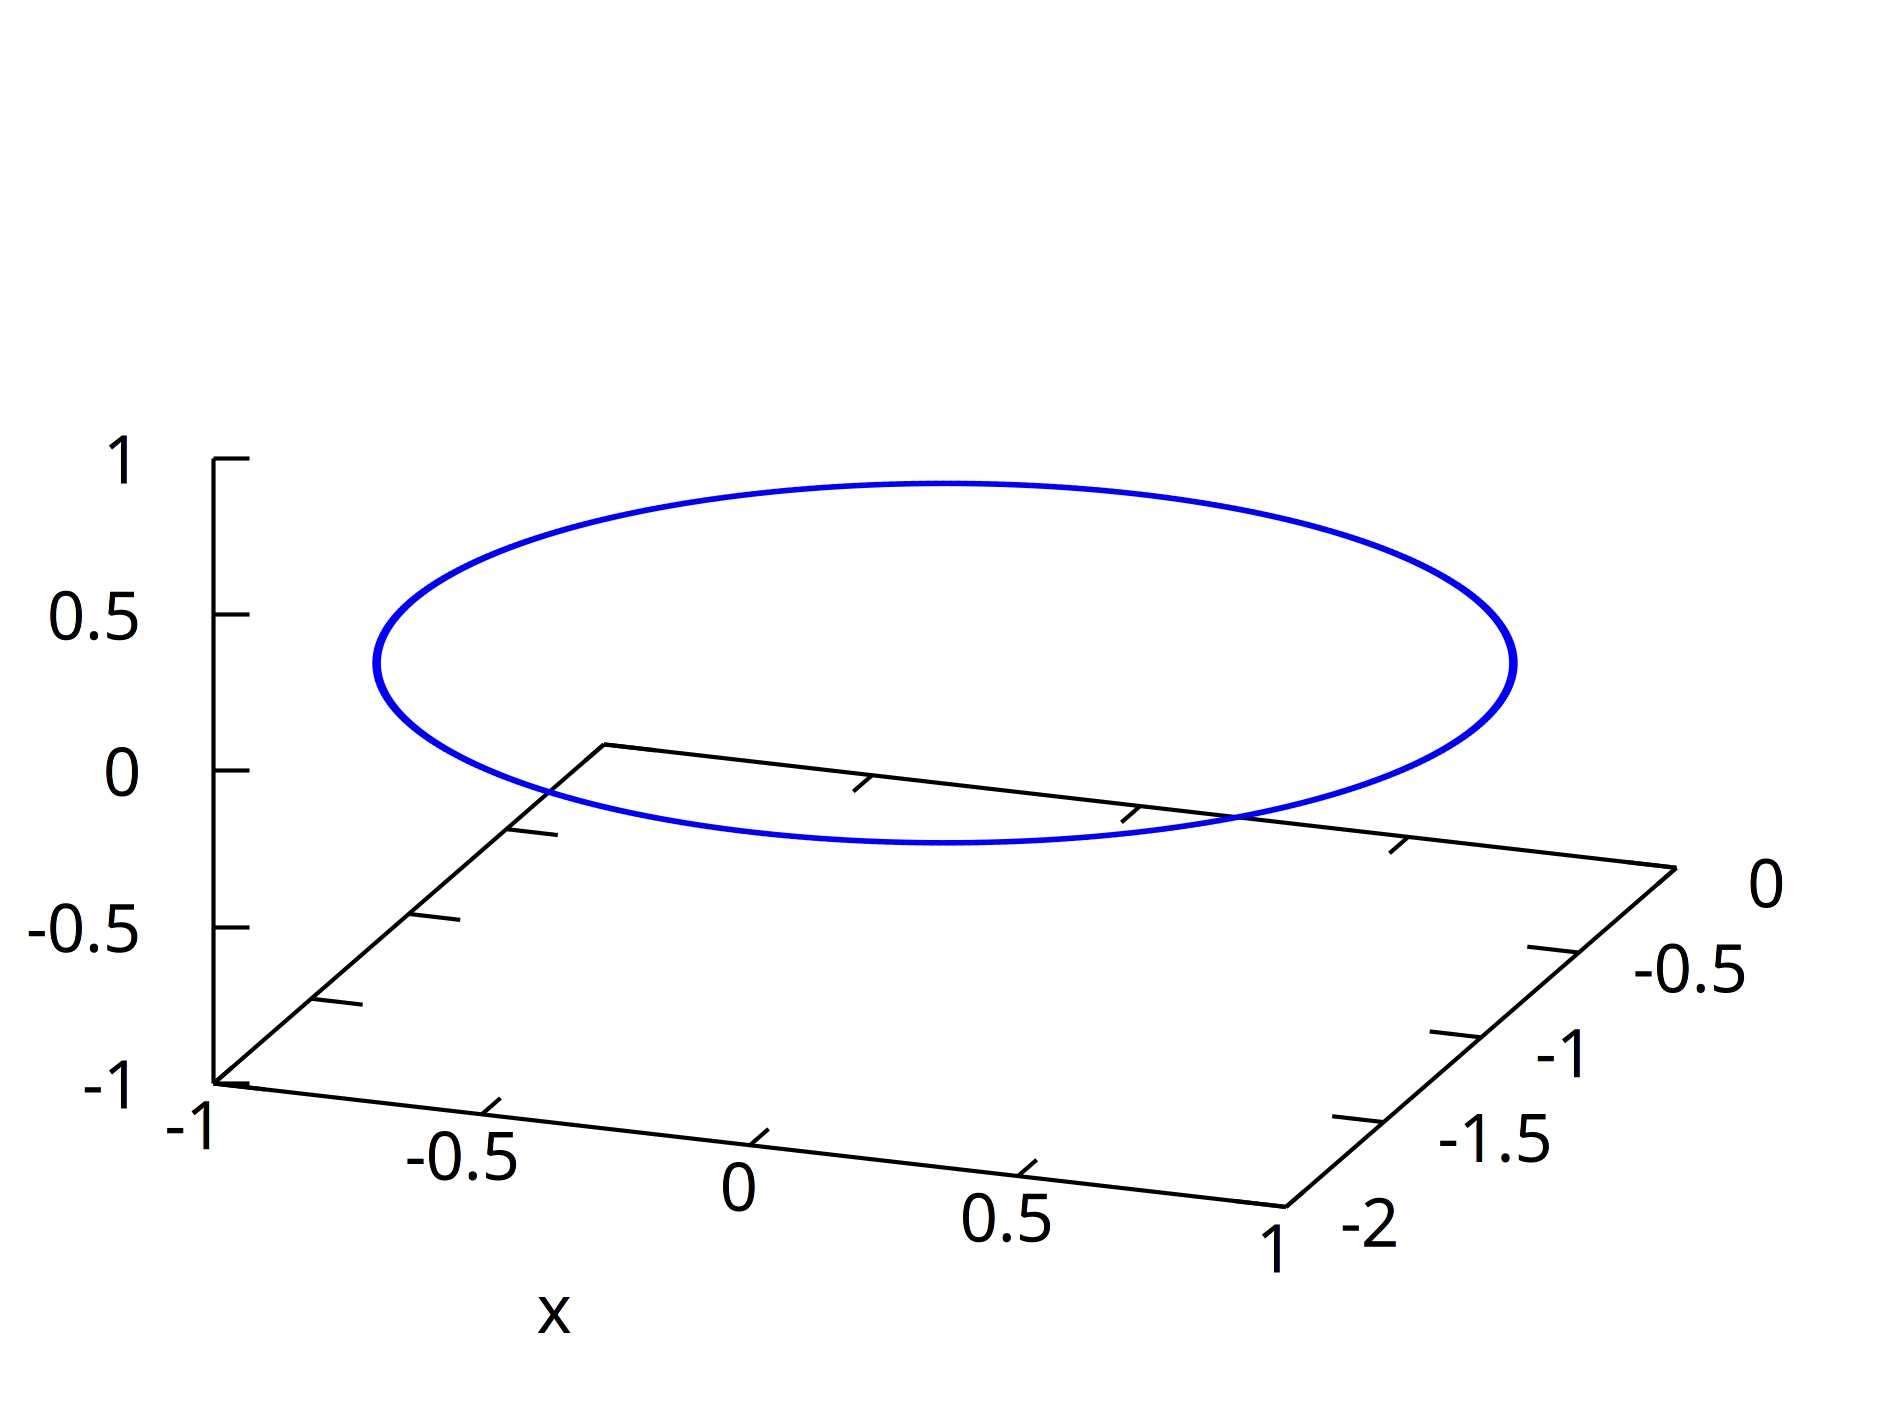
\includegraphics[width=.9\linewidth]{img/3dposizione.png}  
  \caption{Traiettoria della particella}
\end{subfigure}
\begin{subfigure}{.5\textwidth}
  \centering
  % include second image
  \includegraphics[width=.9\linewidth]{img/tempovelocitá.png}  
  \caption{Velocitá particella}
\end{subfigure}
\caption{Velocitá perpendicolare a $\mathbf{B}$}
\end{figure}


\subsection{Confronto Rk2, Rk4 e Boris Pusher}
\begin{figure}[ht]
\begin{subfigure}{.5\textwidth}
  \centering
  % include first image
  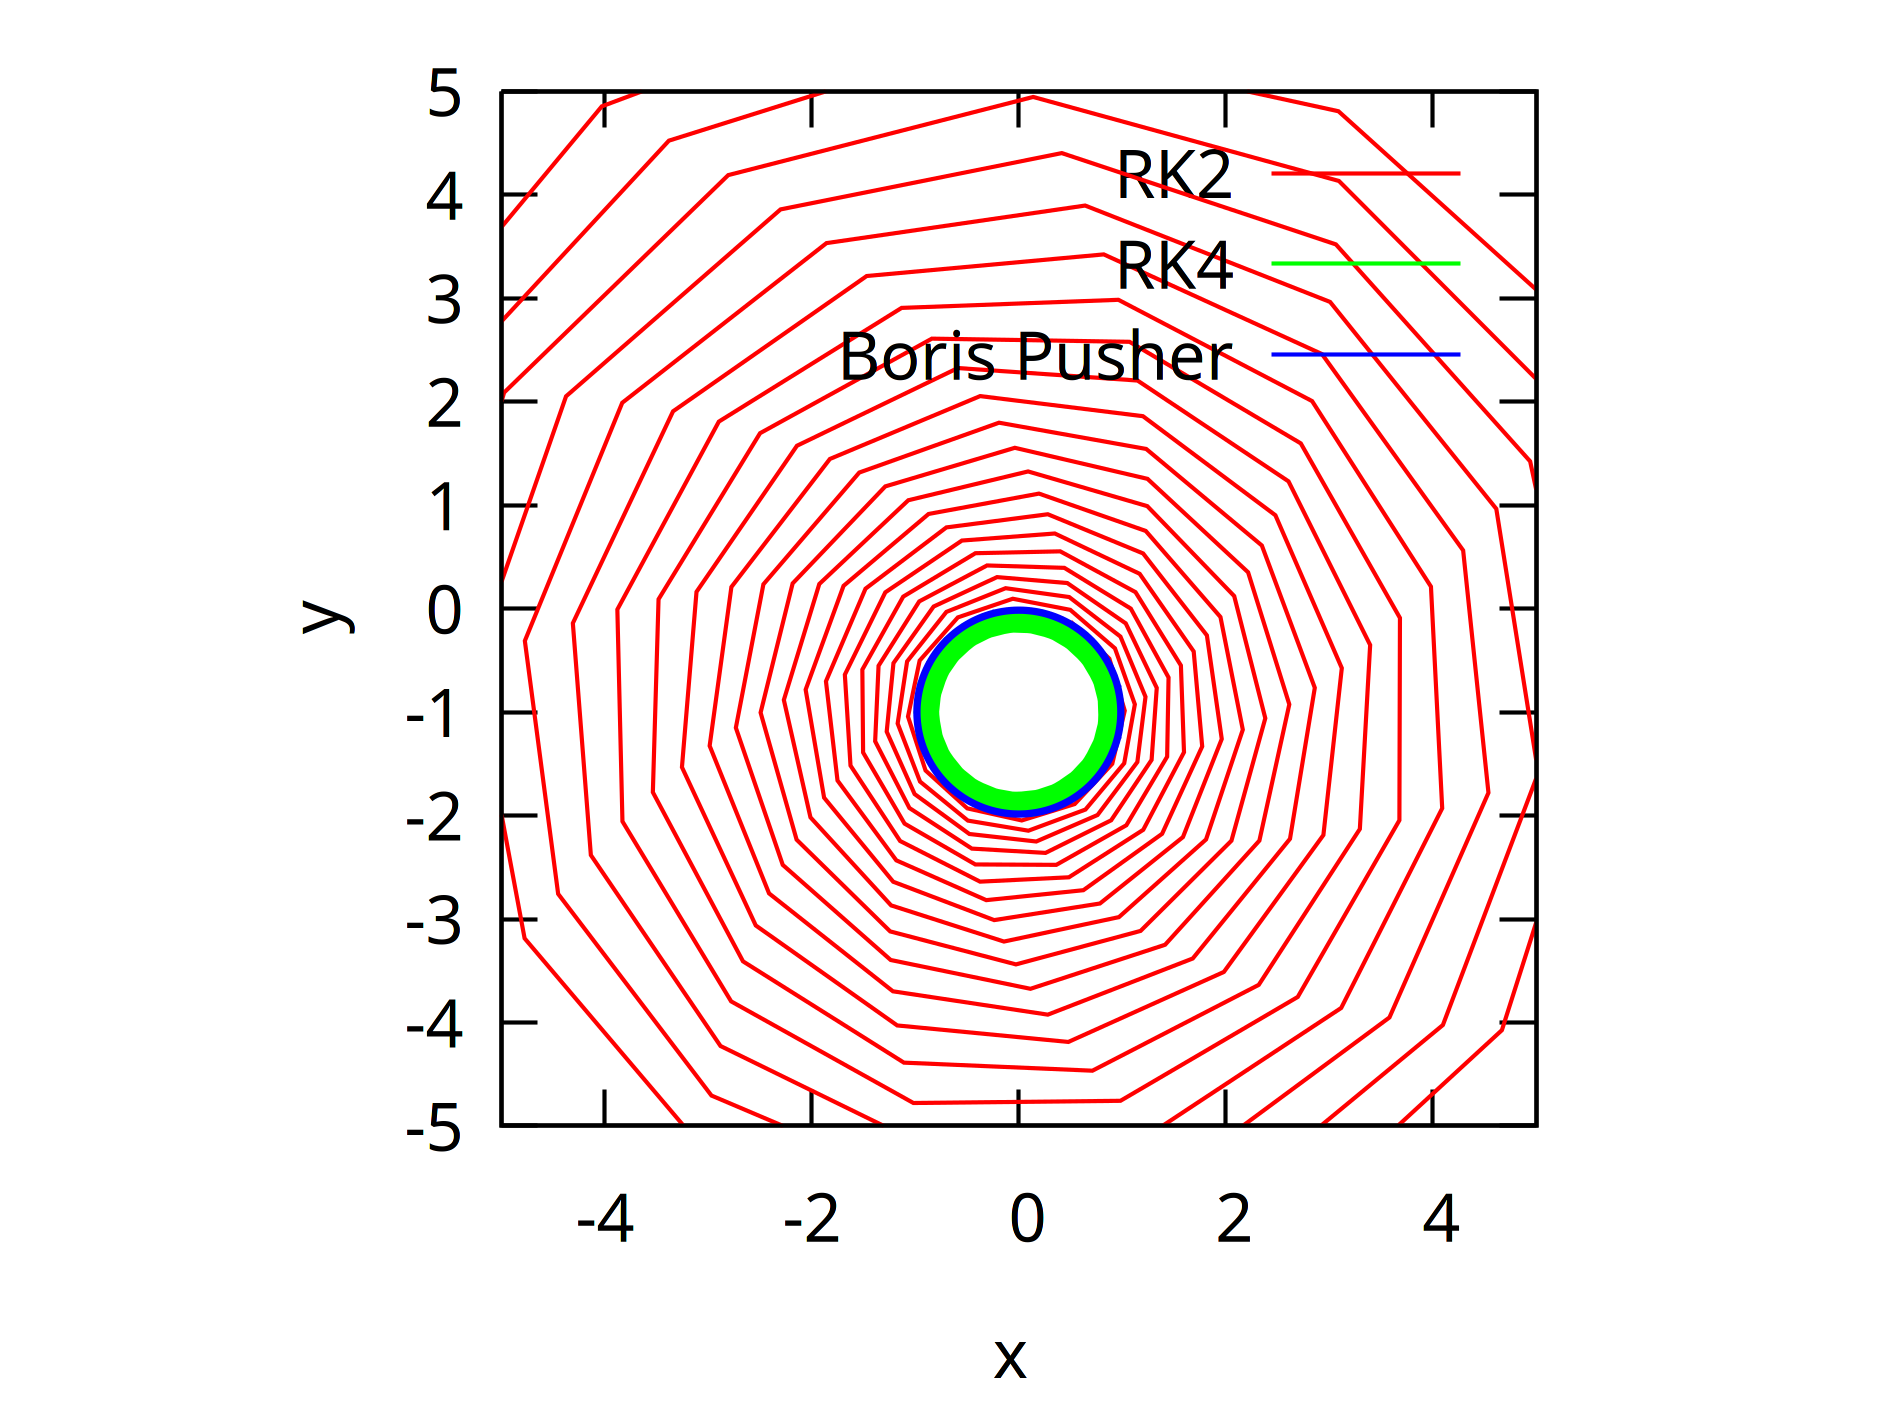
\includegraphics[width=.9\linewidth]{./img/confronto_traiettorie.png}  
  \caption{Confronto tra le traiettorie }
\end{subfigure}
\begin{subfigure}{.5\textwidth}
  \centering
  % include second image
  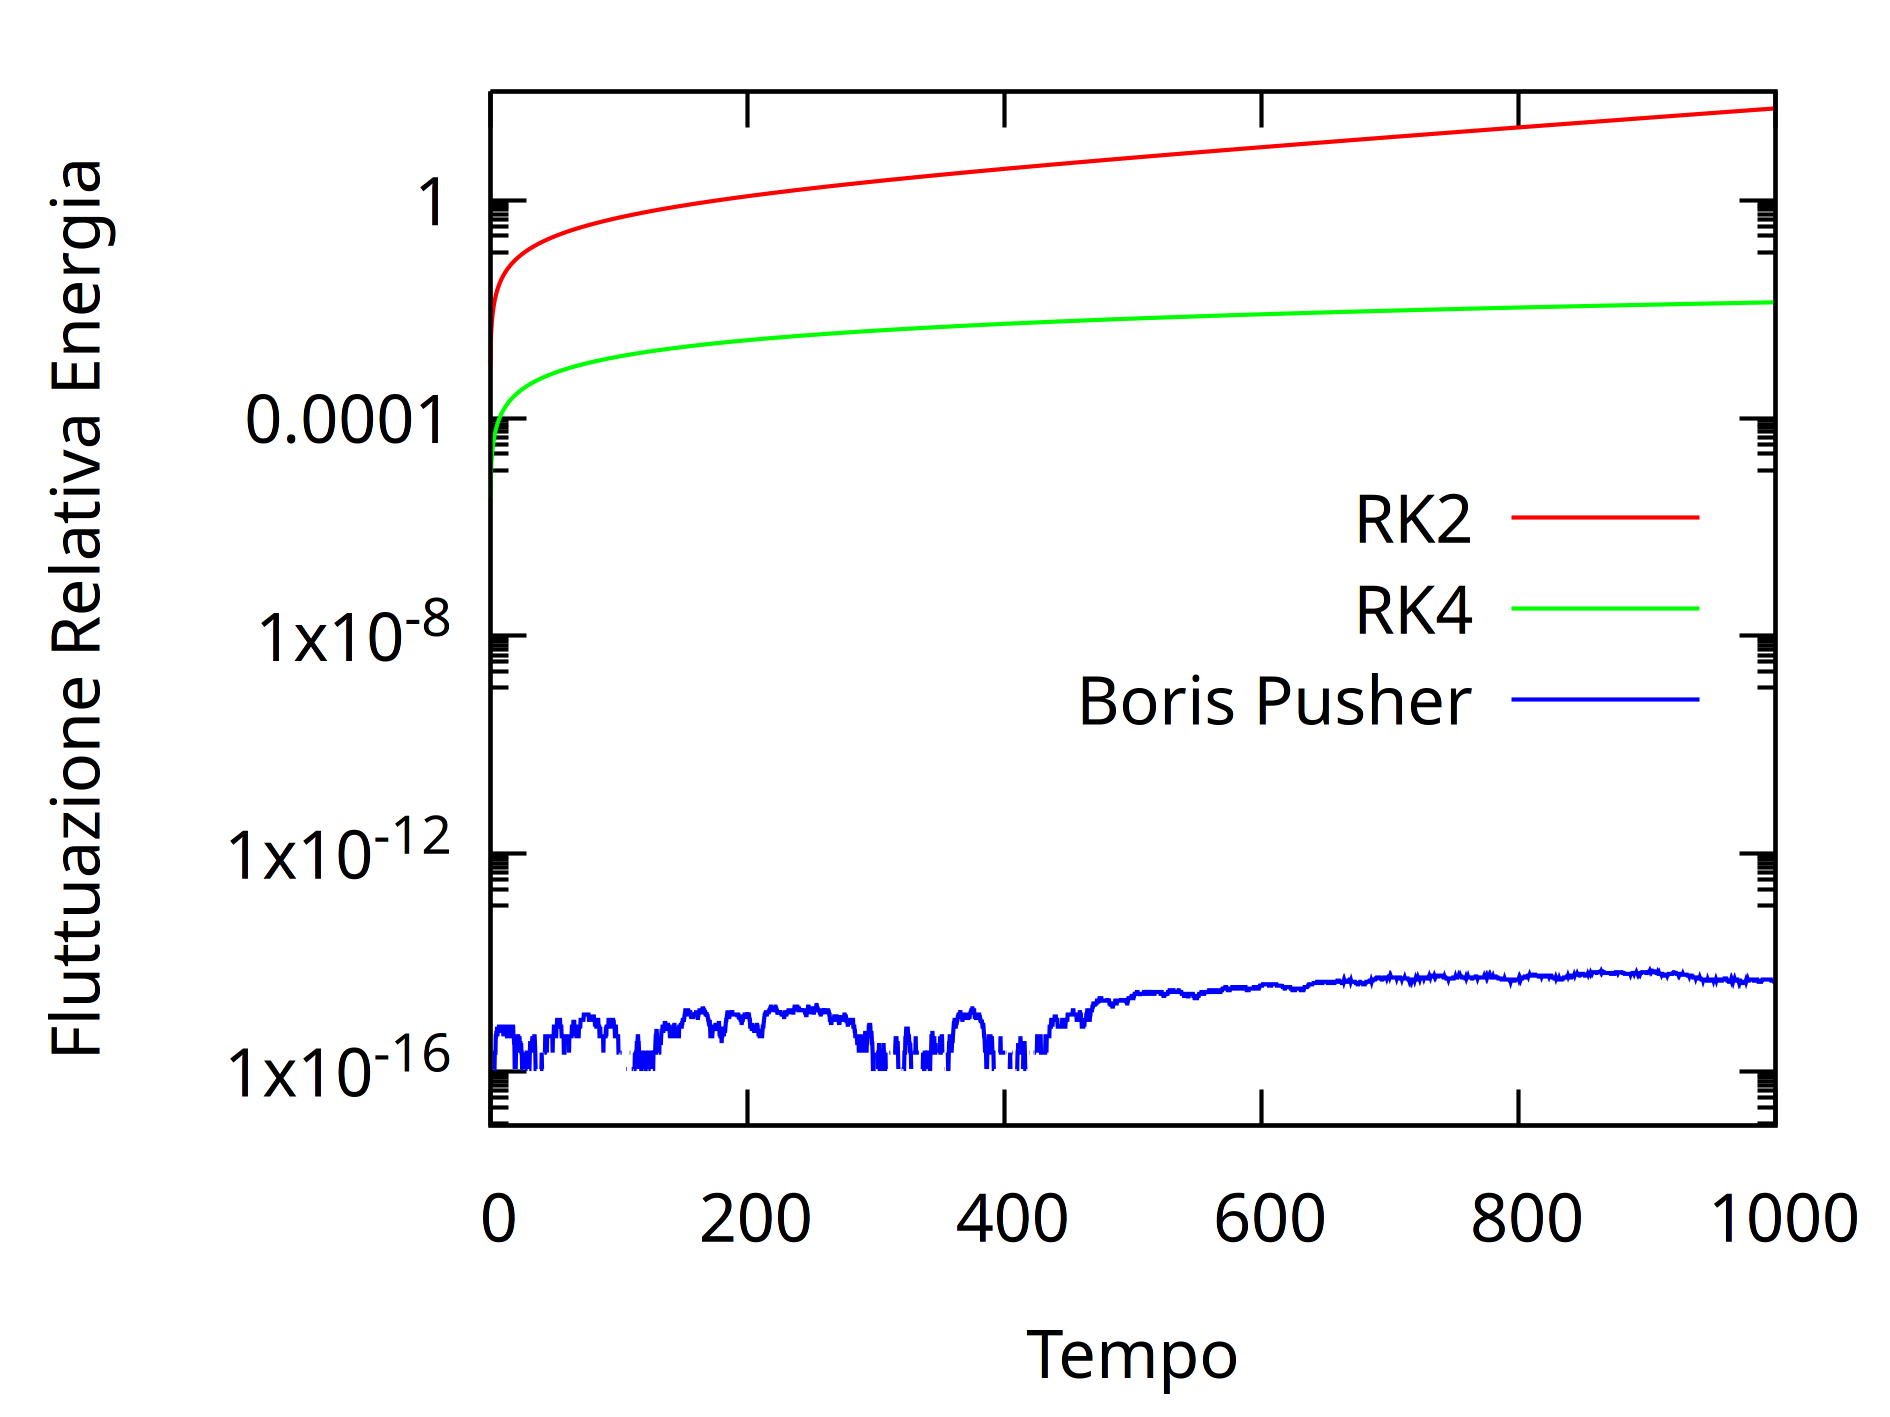
\includegraphics[width=.9\linewidth]{./img/erroreE.png}  
  \caption{Fluttuazione relativa dell'energia totale}
\end{subfigure}
\caption{Confronto tra RK2, RK4 e Boris Pusher con un timestep dt = 0.25 e 1000 step}
\end{figure}
Valuto il diverso comportamento dei tre integratori considerando come varia l'energia della particella durante l'integrazione. 
Infatti il sistema fisico considerato conserva l'energia iniziale per cui mi aspetto che anche la simulazione numerica la conservi. \\ 
$$\Delta E=\frac{|E-E_0|}{E_0} = \frac{|\mathbf{v}^2 - \mathbf{v}_0^2|}{\mathbf{v}_0^2}$$
Valuto l'errore relativo sull'energia considerando soltanto l'energia cinetica della particella in quanto il campo magnetico B non fornisce energia in quanto é sempre perpendicolare alla direzione di spostamento, influisce quindi soltanto sulla direzione della velocitá e non sul modulo.
L' errore per Rk2 e Rk4 raggiunge valori rilevanti e continuerebbe a crescere, mentre l'algoritmo di Boris mantiene un errore trascurabile costante compreso tra a $10^{-16}$ e $10^{-14}$. Verifichiamo  che l'uso di un integratore simplettico permette la conservazione dell'energia iniziale.
Nelle simulazioni seguenti sará implementato l'integratore di Boris.

\section{ExB Drift}
Ora consideriamo il moto di una particella in moto in presenza anche di un campo elettrico E oltre al campo magnetico B.
$$\mathbf{B}=(0,0,B_z) \qquad B_z=1   $$
$$\mathbf{E}=(0,E_y,0) \qquad E_y=0.5 $$
$$
\begin{cases} 
\frac{dv_x}{dt}=v_y B_z \\ 
\frac{dv_y}{dt}=E_y  \\ 
\frac{dv_z}{dt}=0 
\end{cases}
$$

\begin{figure}[ht]
\begin{subfigure}{.5\textwidth}
  \centering
  % include first image
  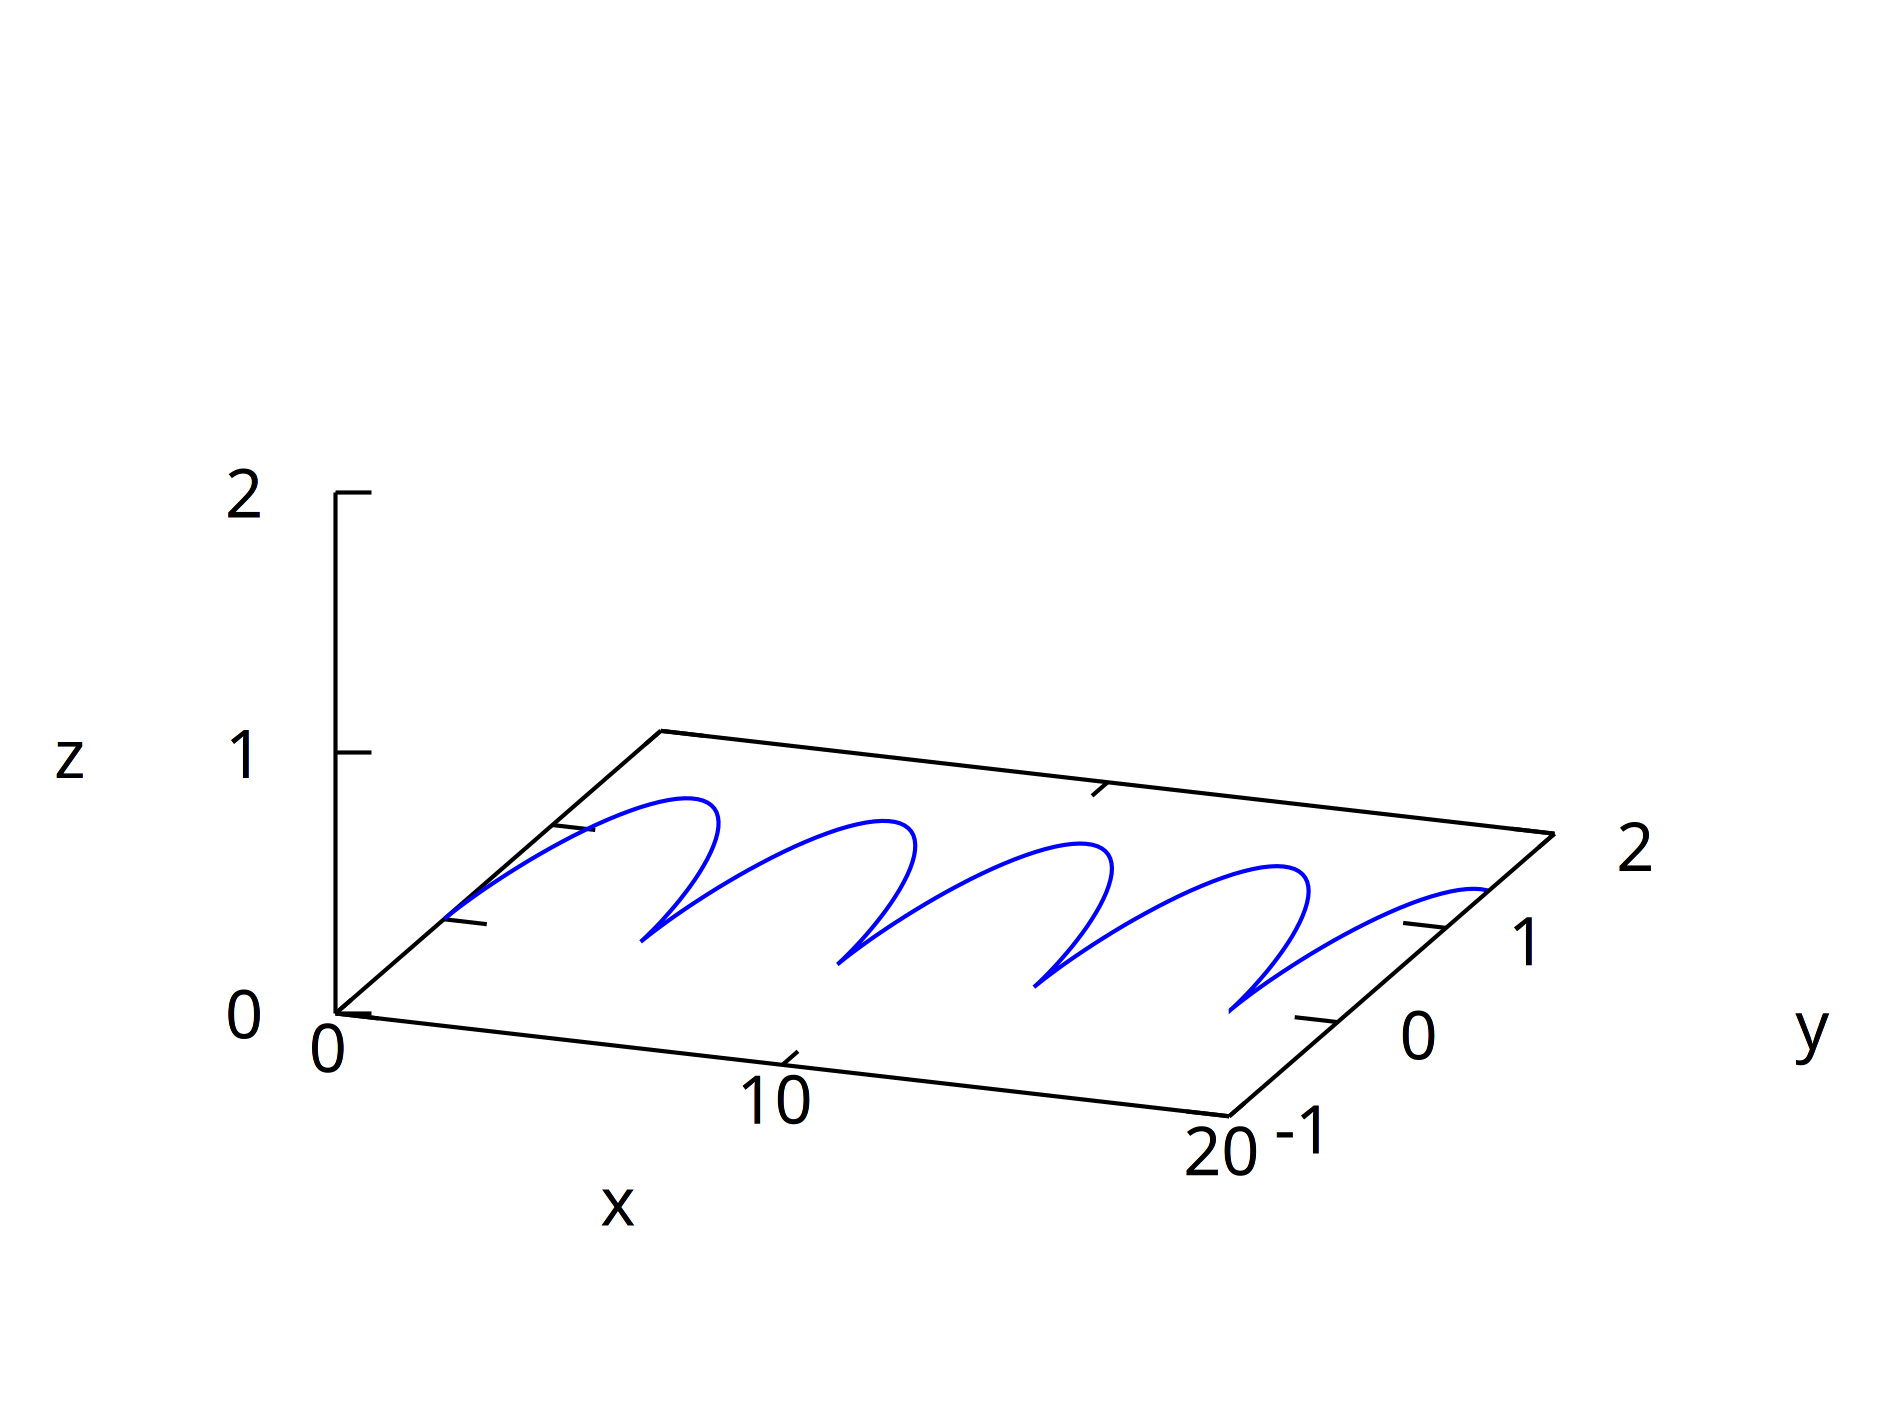
\includegraphics[width=.9\linewidth]{img/3dposizionedrift.png}  
  \caption{Traiettoria nello spazio 3d}
\end{subfigure}
\begin{subfigure}{.5\textwidth}
  \centering
  % include second image
  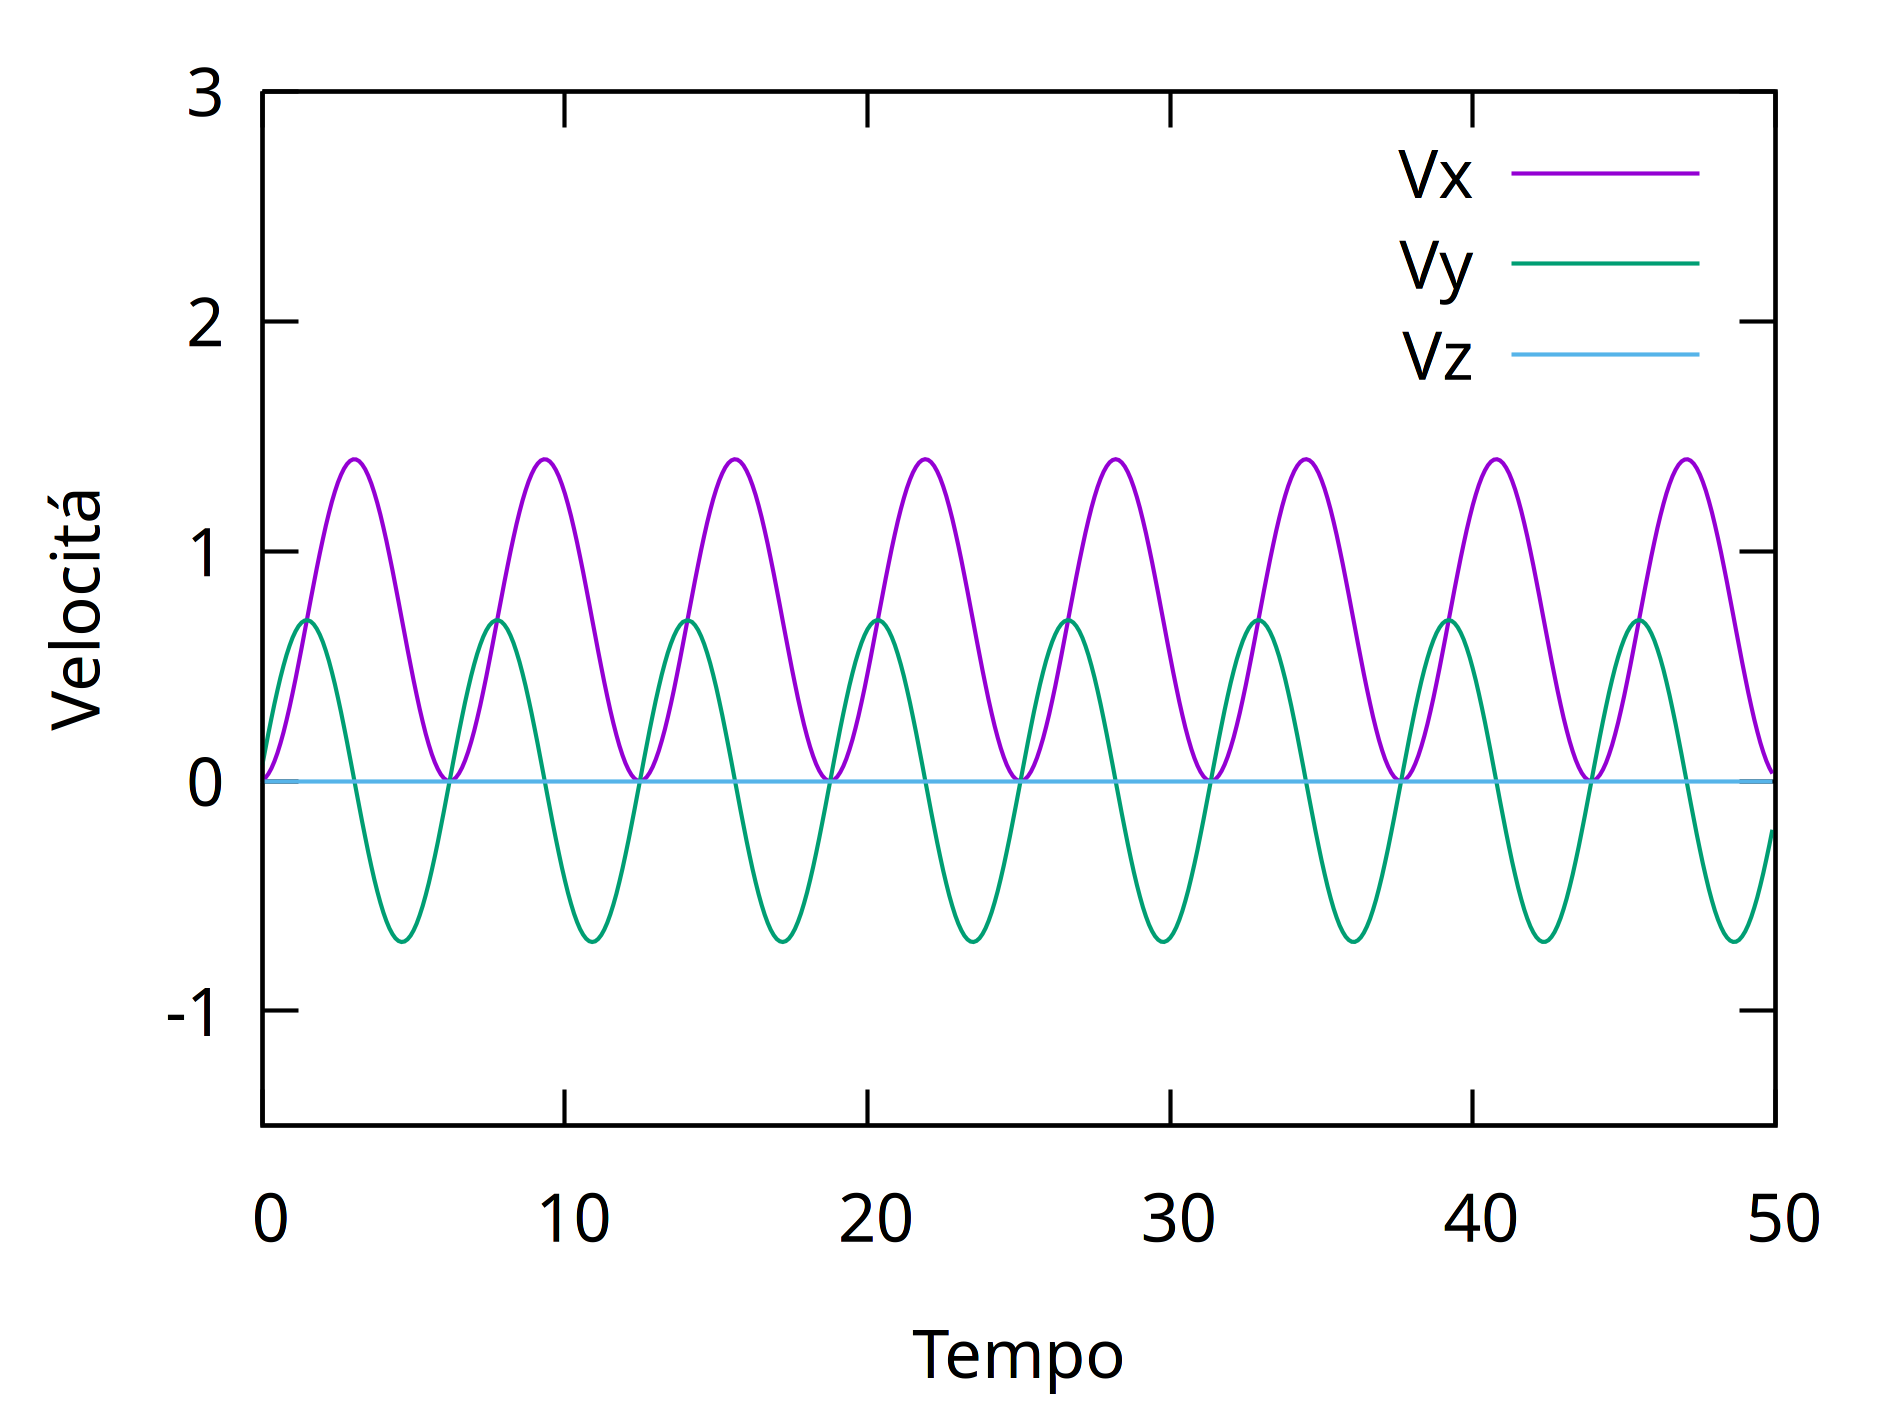
\includegraphics[width=.9\linewidth]{img/vdrift.png}  
  \caption{Velocitá }
\end{subfigure}
\caption{ExB Drift}
\end{figure}%
La traiettoria della particella segue una cicloide lungo la direzione x. Il moto é inaspettato avendo un campo elettrico agente in direzione $y$ che accellera costantemente la particella lungo questa direzione.\\\
In realtá, quando la velocitá della particella aumenta cresce anche la forza risultante dall'interazione con $\mathbf{B}$, sempre normale rispetto alla traiettoria.
Infatti la carica ferma nell'origine subisce un accelerazione lungo y dovuta a $\mathbf{E}$. Appena la carica inizia a muoversi la forza magnetica agisce nella direzione normale alla traiettoria. Questo fino alla fine del periodo dove la forza risultante é nulla, per cui la carica si ferma e il moto si ripete periodico.

\section{10k Particelle}
Posiziono $N = 10^4 $ particelle in un quadrato $L \times L$ con posizione e velocitá uniformemente distribuite. In particolare la velocitá di ognuna sará $|v|=0.1$ e direzione casuale ottenuta con un angolo casuale tra $0$ e $2\pi$.\\
Le particelle sono immerse in un campo elettrico e magnetico:
$$\vec{E}=\left(0,0,\frac{1}{2} \right)$$
$$\vec{B}=\left(\frac{y}{L},\frac{x}{L},0\right) $$ 
Scrivo le equazioni del moto:
$$
\begin{cases} 
\frac{dv_x}{dt}= 0 \\ 
\frac{dv_y}{dt}= 0 \\ 
\frac{dv_z}{dt}= \frac{1}{2} + \frac{x}{L}v_x - \frac{y}{L}v_y 
\end{cases}
$$
Le particelle compiono un moto peculiare, infatti le particelle che si trovano nella zona centrale del quadrato, vengono accellerate magiormente verso $z$ dando effetto a una sorta di getto di particelle. Mentre alla base del cono si possono osservare delle oscillazioni concentriche.


\begin{figure}
\centering
\begin{subfigure}{0.33\textwidth}
    \centering
    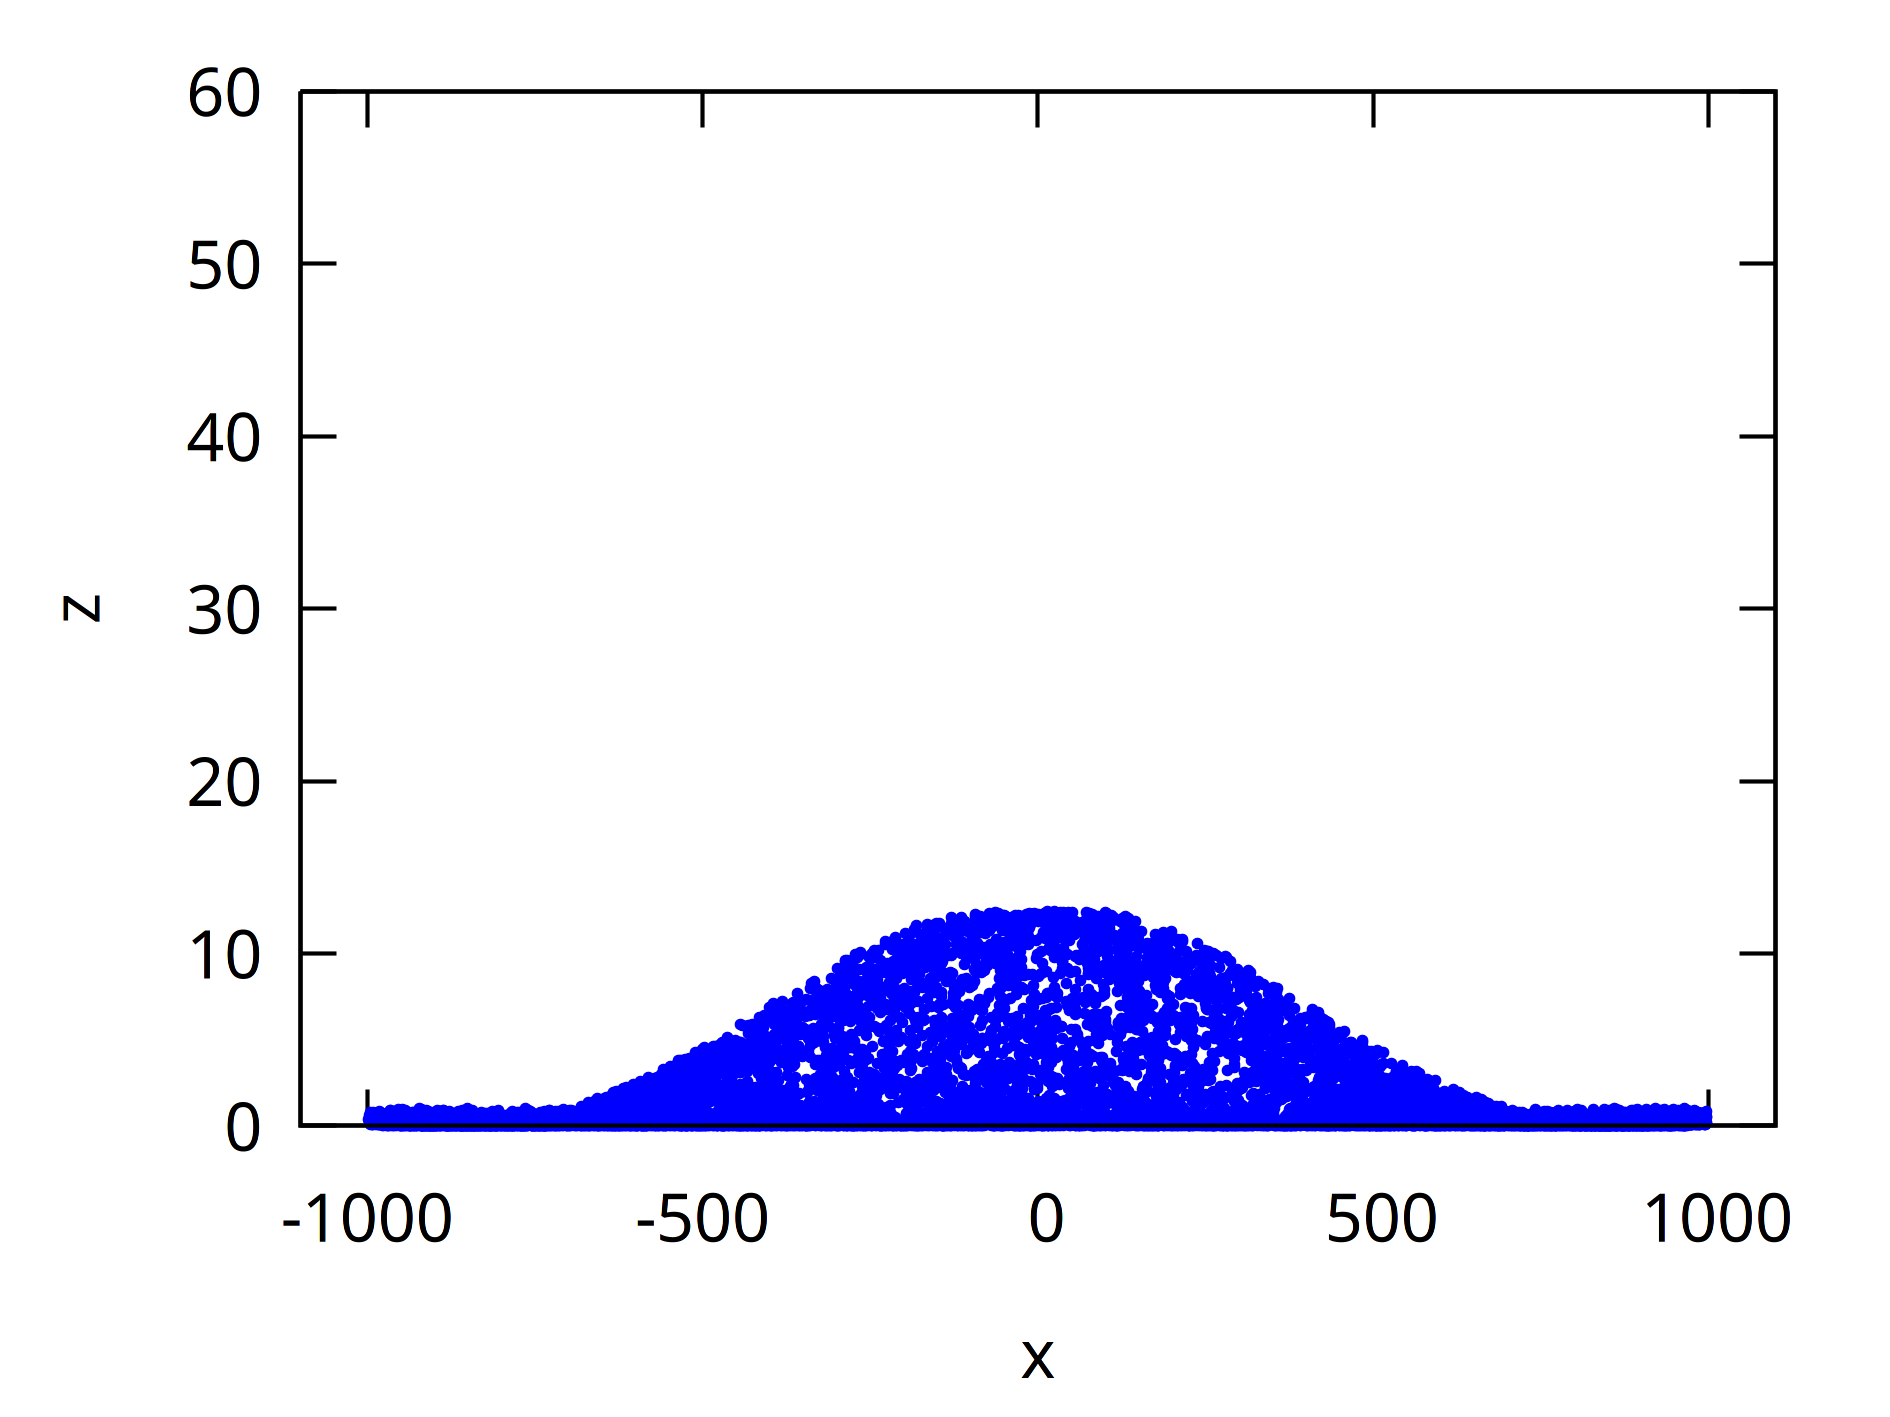
\includegraphics[width=1.\textwidth]{img/lateral_70.png}
    \subcaption{t = 70 }
\end{subfigure}%
\begin{subfigure}{0.33\textwidth}
    \centering
    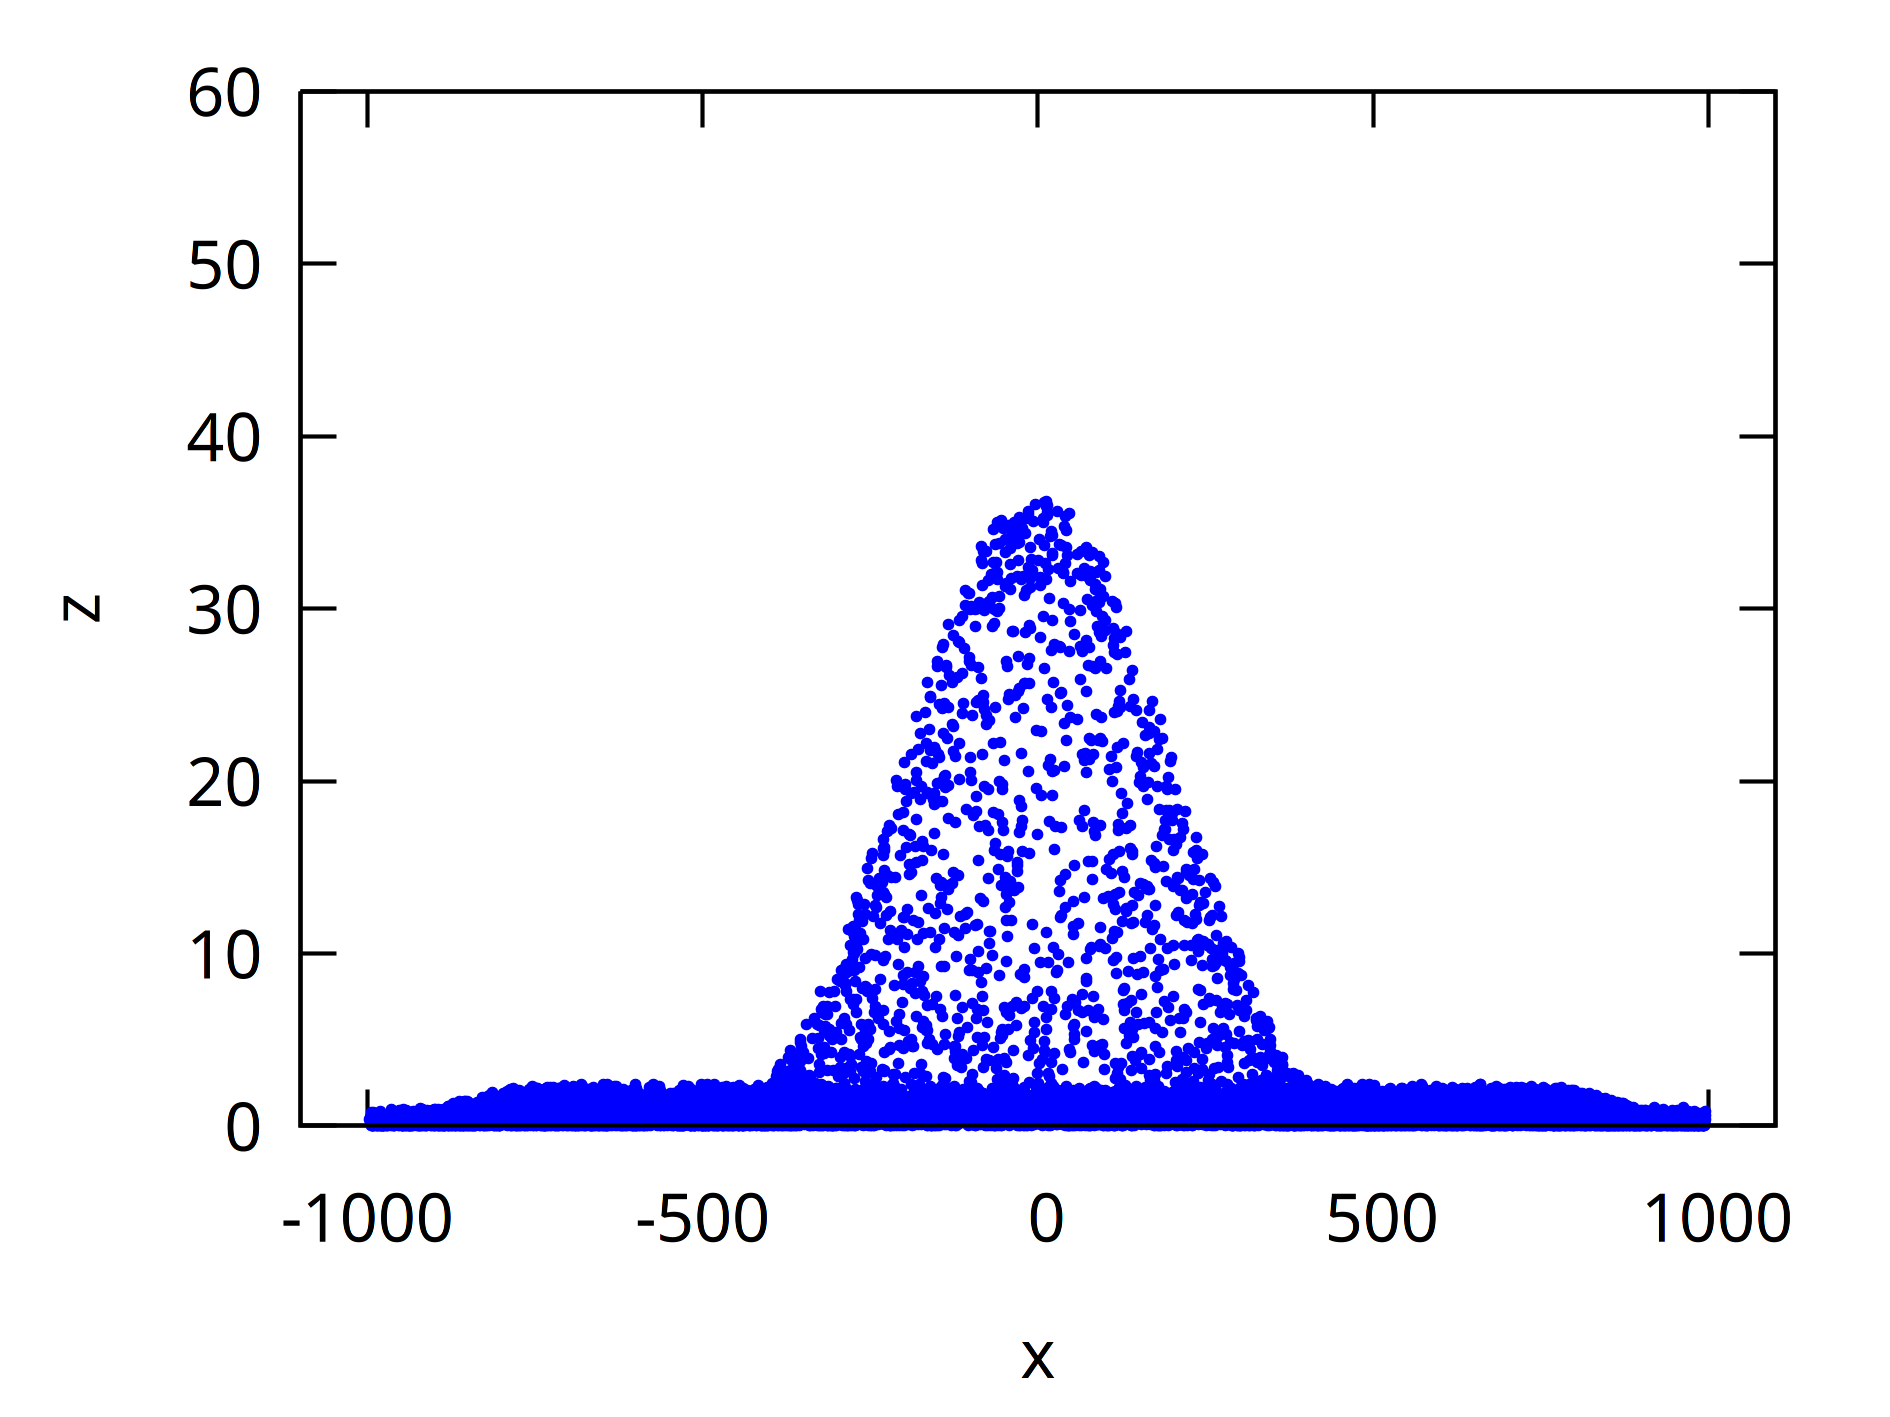
\includegraphics[width=1.\textwidth]{img/lateral_120.png}
    \subcaption{t = 120 }

\end{subfigure}%
\begin{subfigure}{0.33\textwidth}
    \centering
    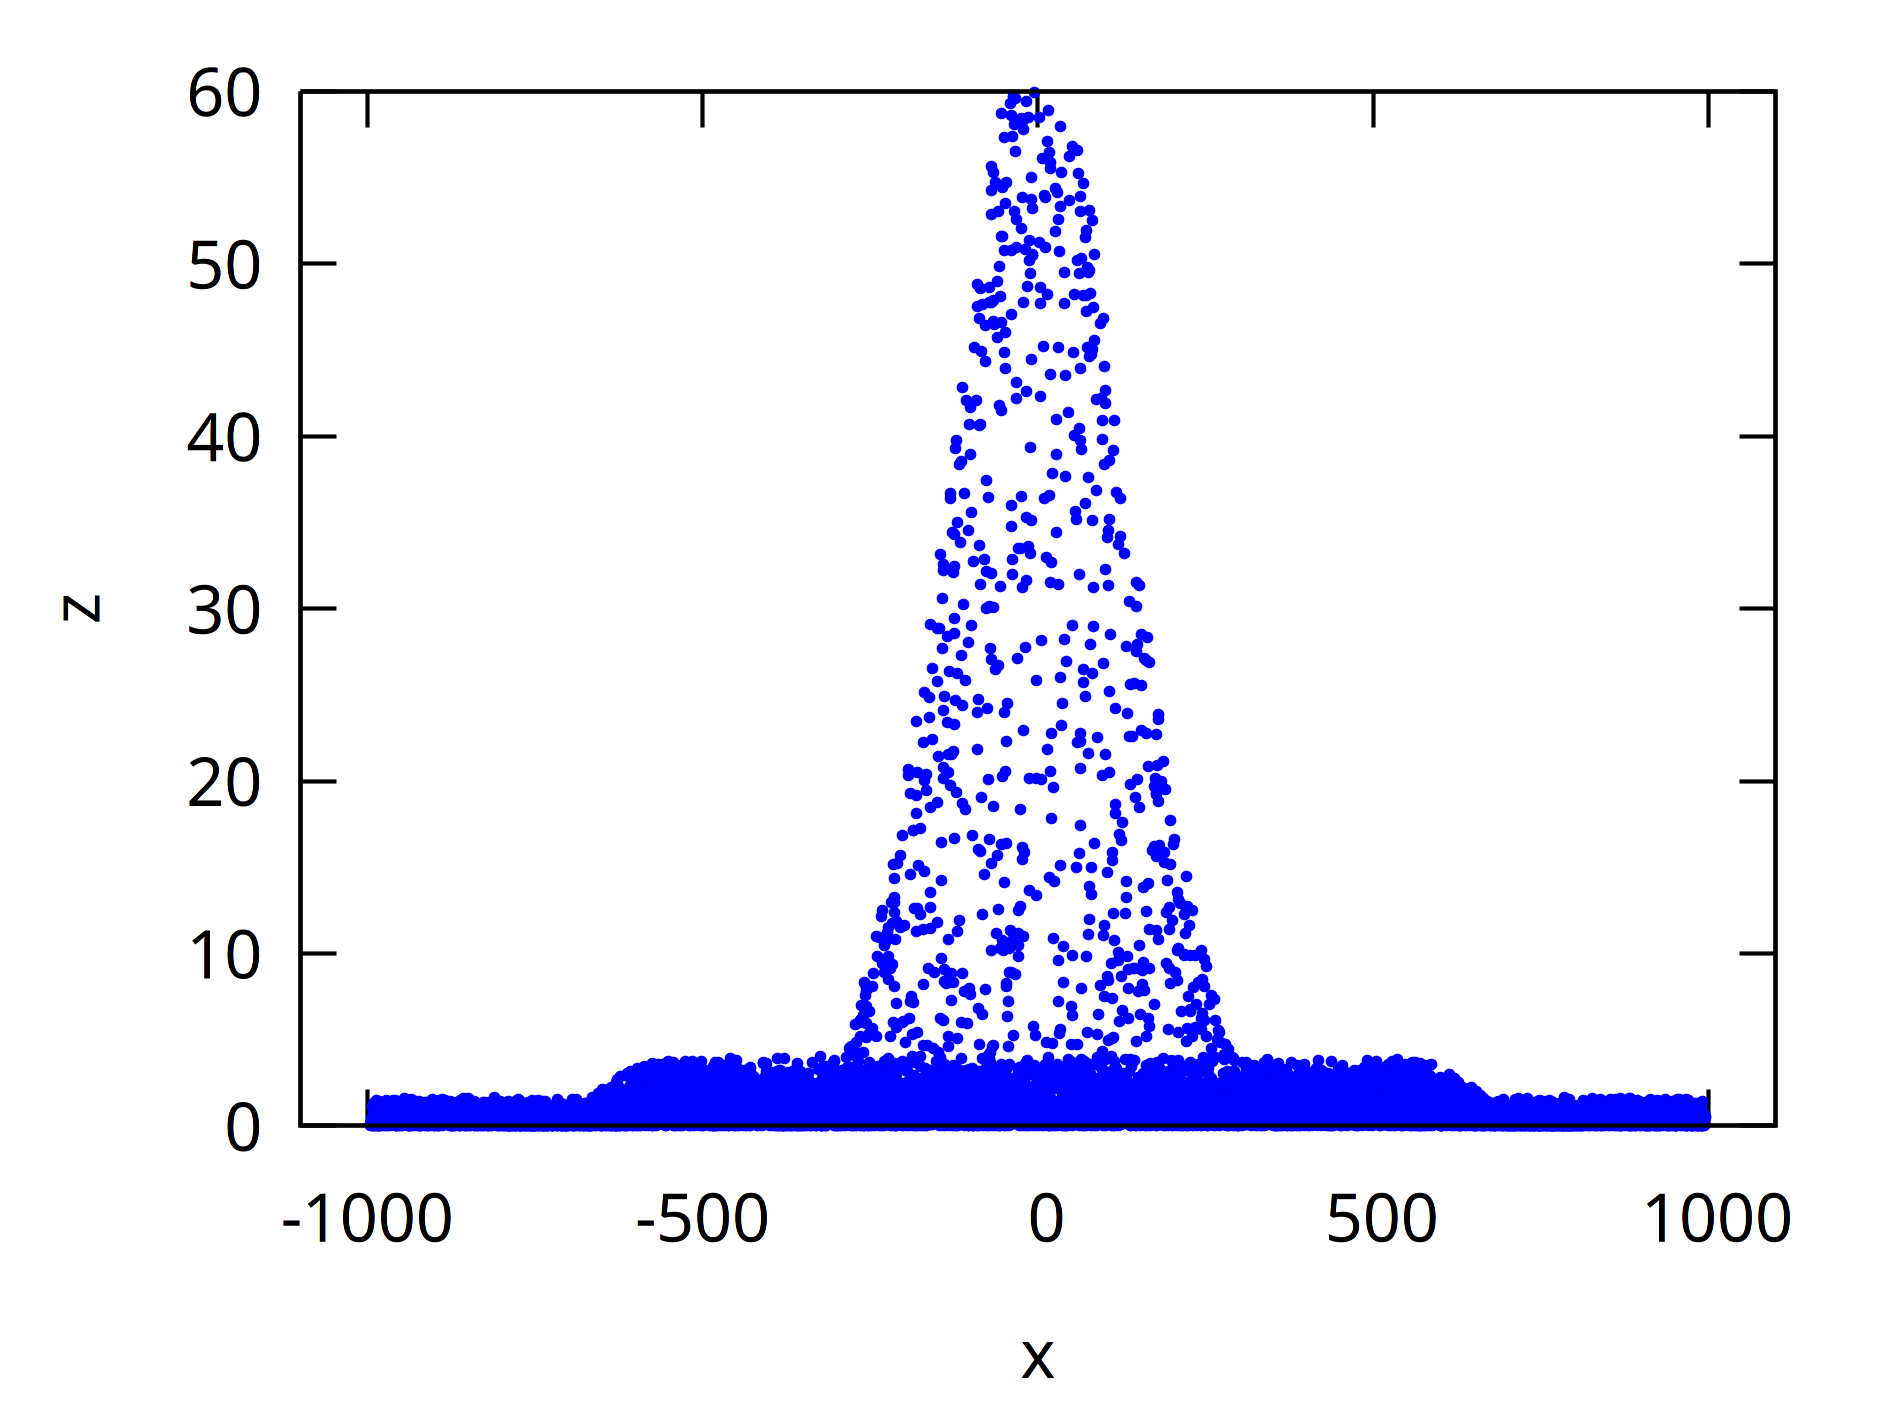
\includegraphics[width=1.\textwidth]{img/lateral_160.png}
    \subcaption{t = 160 }
\end{subfigure}



\begin{subfigure}{0.33\textwidth}
    \centering
    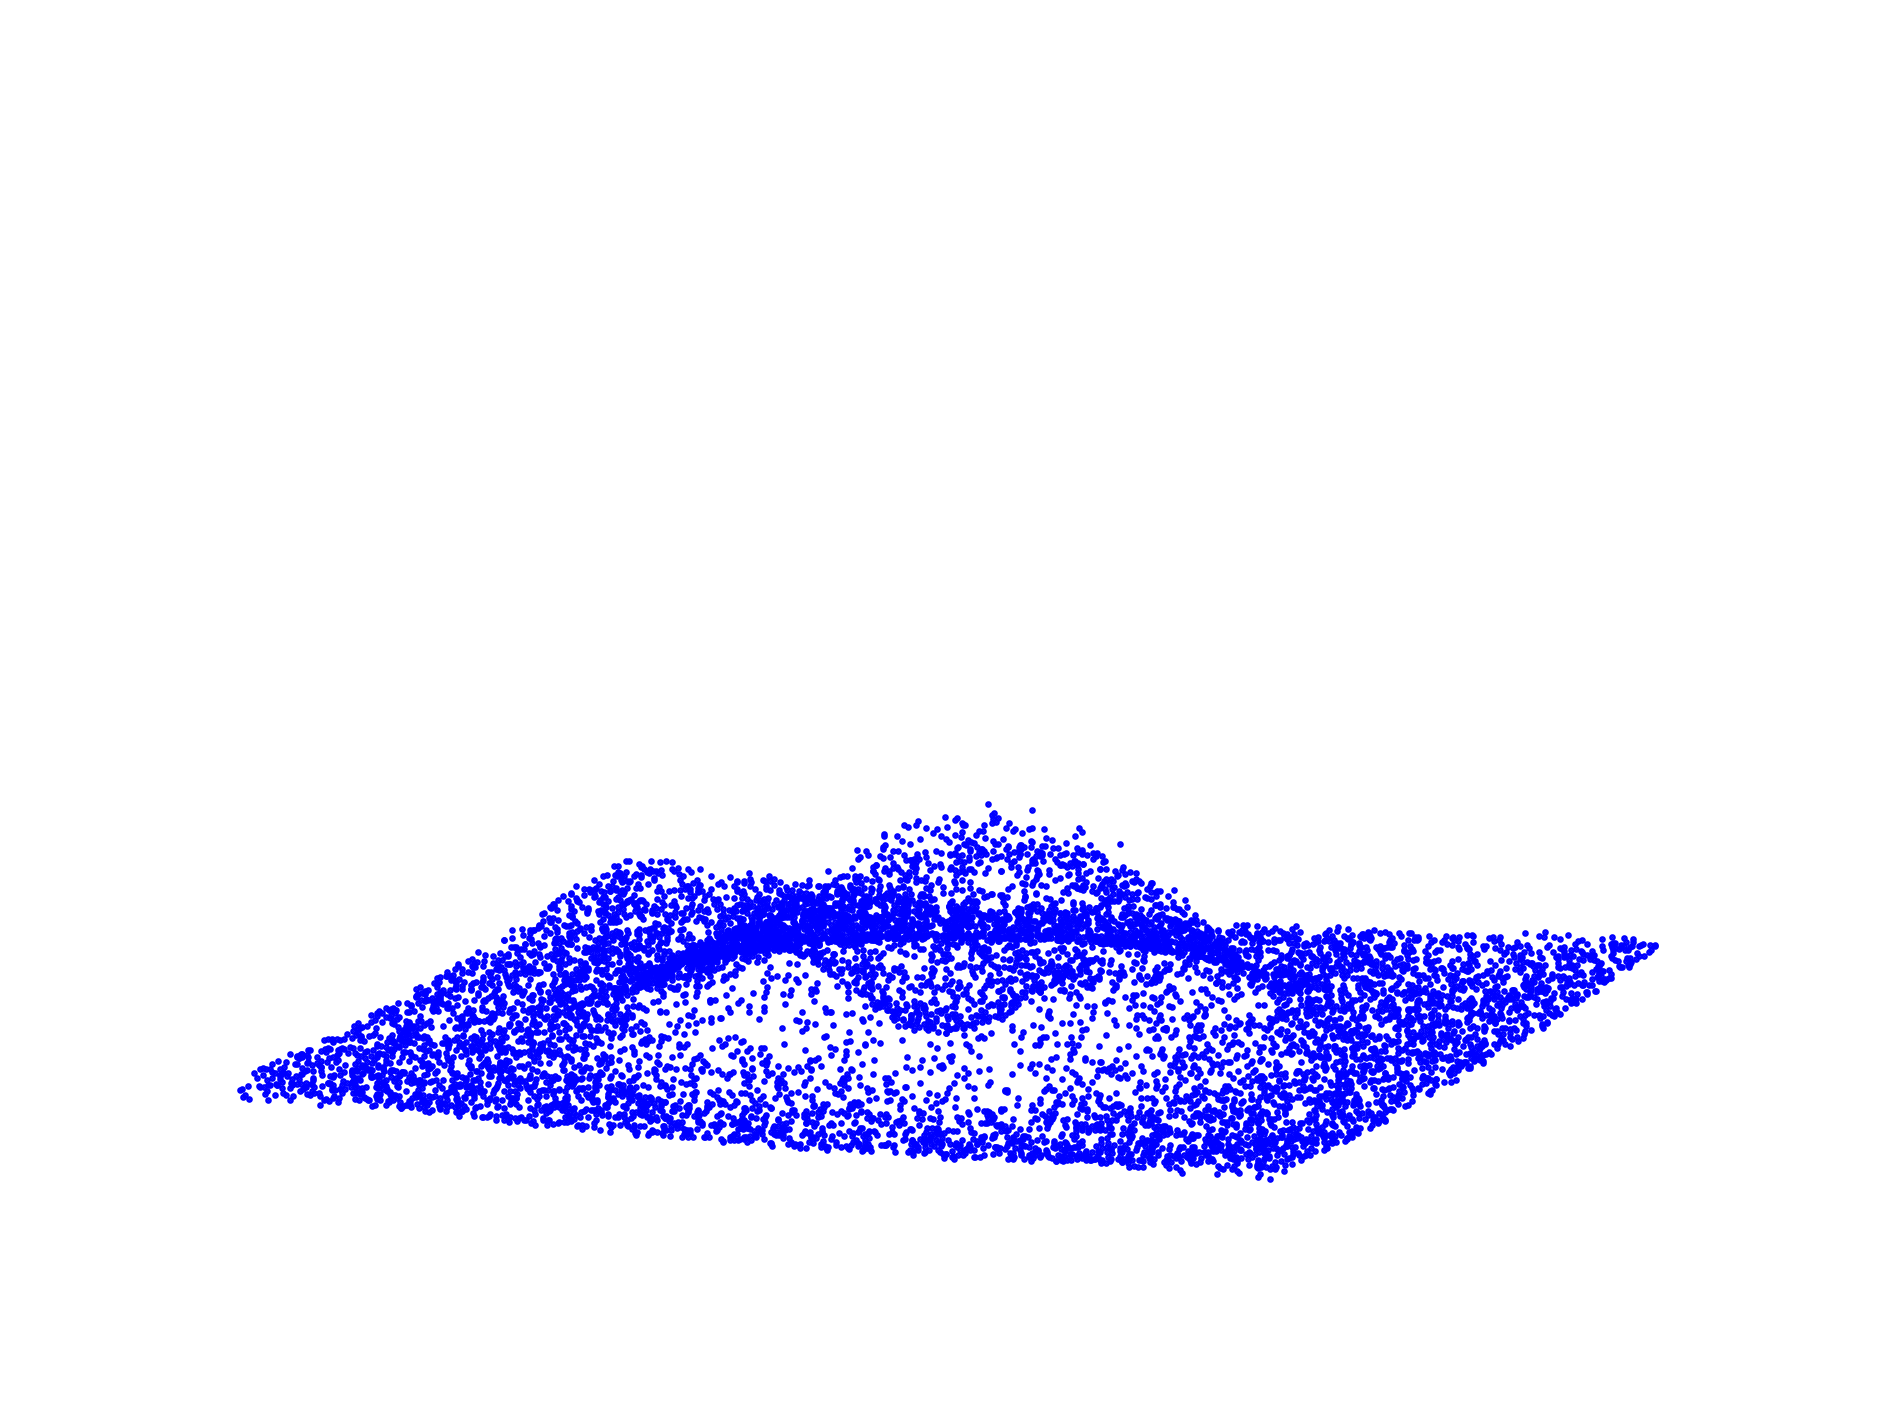
\includegraphics[width=1.\textwidth]{img/distrib_70.png}
    \subcaption{t = 70 }
\end{subfigure}%
\begin{subfigure}{0.33\textwidth}
    \centering
    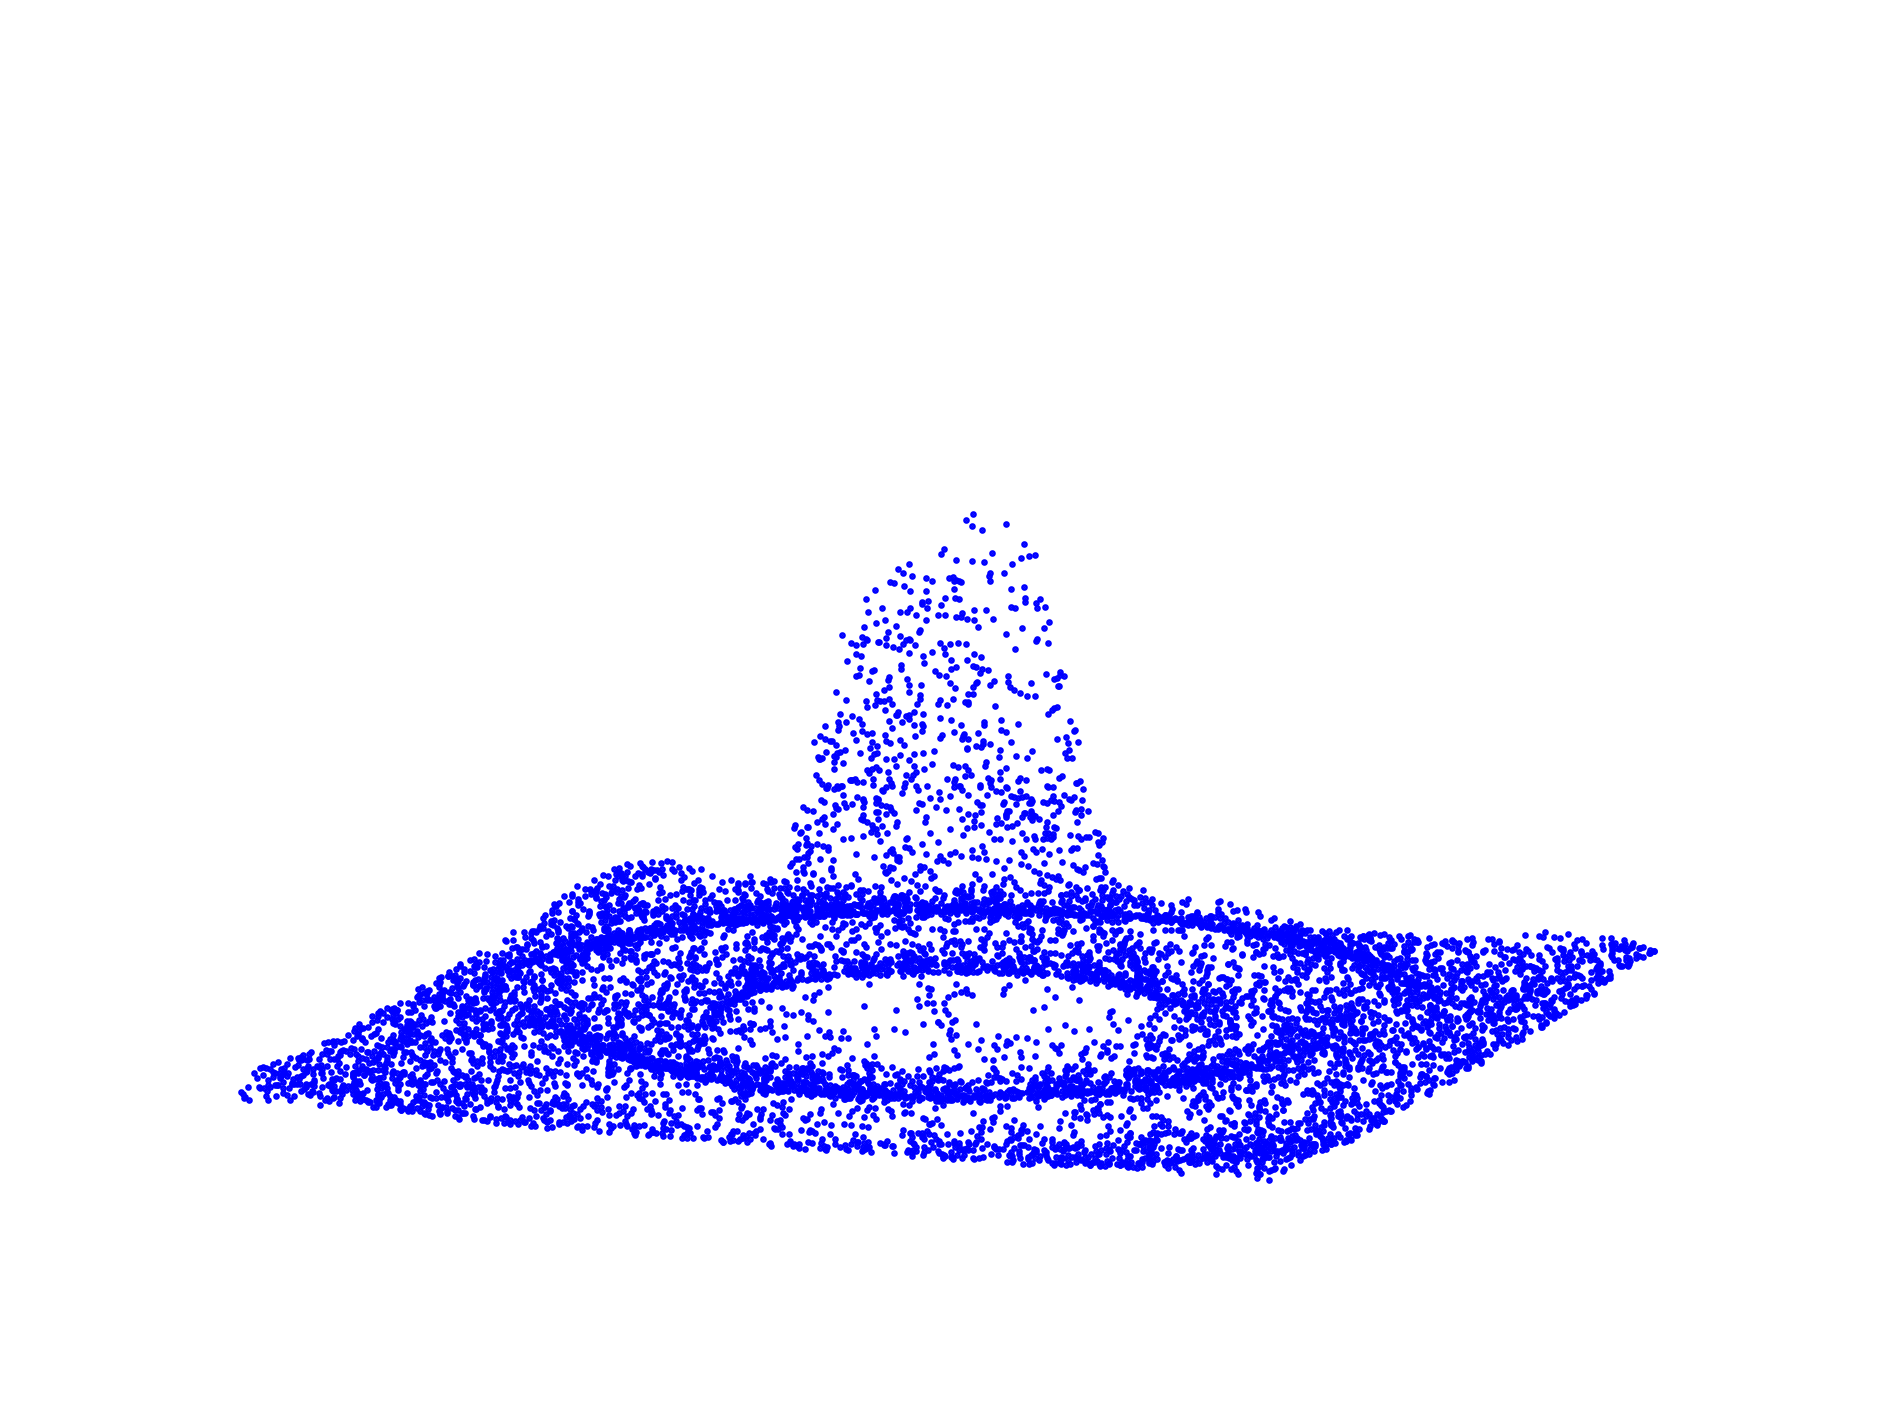
\includegraphics[width=1.\textwidth]{img/distrib_120.png}
    \subcaption{t = 120 }
\end{subfigure}%
\begin{subfigure}{0.33\textwidth}
    \centering
    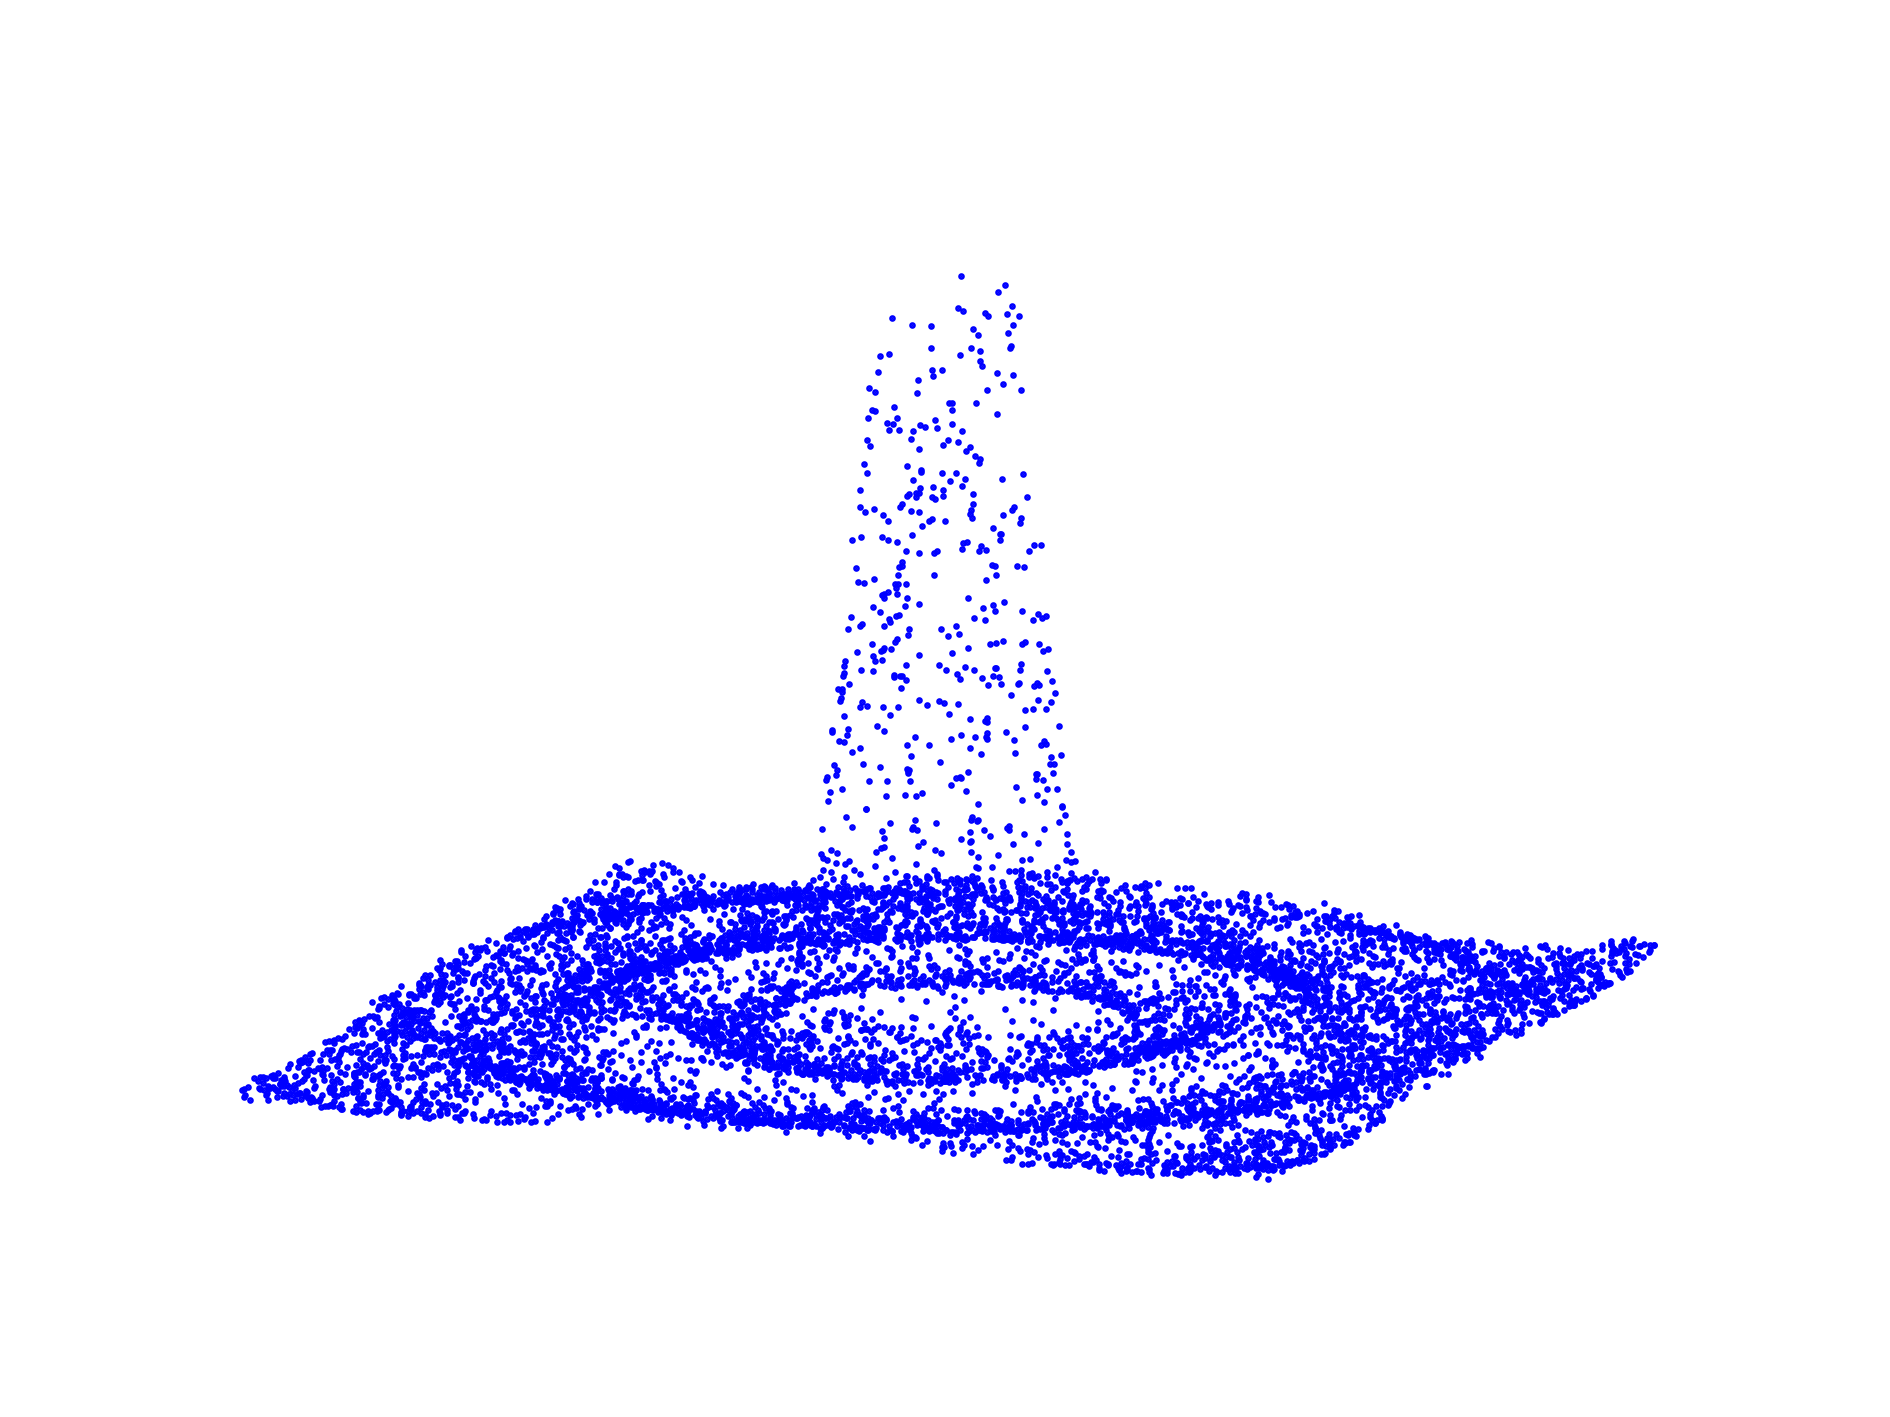
\includegraphics[width=1.\textwidth]{img/distrib_160.png}
    \subcaption{t = 160 }
\end{subfigure}
\caption[short]{Posizioni delle particelle in tre diversi istanti}
\end{figure}


\section{Conclusioni}
Abbiamo considerato tre diversi esempi di particelle in campi elettrici e magnetici, in particolare per l'ultimo caso la simulazione numerica ci ha permesso di comprendere la dinamica non banale del sistema.
